\section{Постановка задачи детектирования фазоманипулированного сигнала с расширенным спектром}
\label{sec1_acq_algo}

\subsection{Постановка задачи поиска сигнала}
В данной работе рассматриваются задачи повышения рабочих характеристик приемников спутниковой навигационной системы
(СНС) GPS, поэтому целесообразно
отразить основные модули этой системы рисунок \ref{pic:sec1_gnss_system}.
\begin{figure}[H]
\center\scalebox{1}{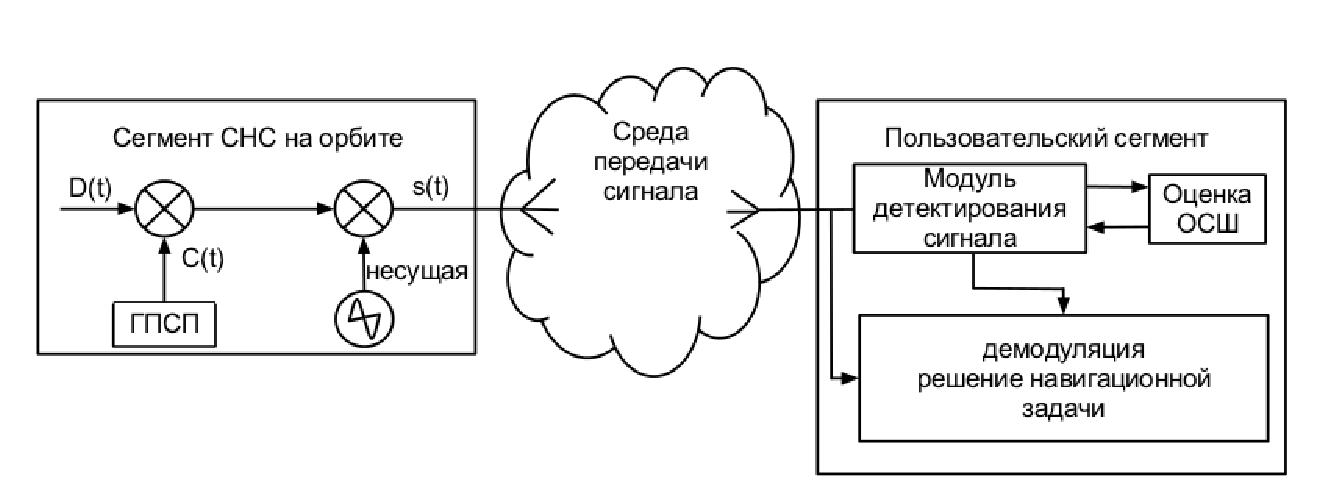
\includegraphics[width=1\linewidth]{sec1gnss_system.eps}}
\caption{структутраная схема СНС GPS}
\label{pic:sec1_gnss_system}
\end{figure}

В систему СНС GPS входят космический сегмент, наземный сегмент (на рисунке \ref{pic:sec1_gnss_system} не
отражен), а так же пользовательский сегмент. В космический сегмент входит спутниковая группировка, в 
наземный - станции управления, в пользовательский - все устройства принимающие сигнал от СНС GPS.

В данной работе рассматривается только пользовательский сегмент. В частности, модули детектирования сигнала,
а так же модули оценки ОСШ принятого сигнала. Далее рассмотрены несколько алгоритмов детектирования сигнала,
а так же алгоритмов оценки ОСШ. Но до рассмотрения алгоритмов обработки сигнала, целесообразно кратко 
отразить свойства, а так же методы модулирования сигналов применяемых в СНС GPS.

\subsection{Модель сигнала и помех СНС GPS}
В системе СНС GPS применяются широкополосные сигналы (ШПС).
ШПС - сигналы, ширина полосы, используемой для передачи сигнала, которых
намного шире минимальной, необходимой для передачи данных \cite{sklyar}. Система связи считается системой с расширенным
спектром в следующих случаях \cite{sklyar}:

\begin{enumerate}
	\item Используемая полоса значительно шире минимальной, необходимой для передачи данных.
	\item Расширение спектра производится с помощью так называемого расширяющего (кодового) сигнала,
		который не зависит от передаваемой информации.
	\item Восстановление исходных данных ("сужение спектра") осуществляется путем сопостовления полученного
		сигнала и синхронизированной копии расширяющего сигнала
\end{enumerate}
Так же подобные сигналы называют:
\textquotedblleftсложными\textquotedblright,
\textquotedblleftшумоподобными\textquotedblright,
\textquotedblleftпсевдослучайными\textquotedblright,
\textquotedblleftсложными-дискретными\textquotedblright,
\textquotedblleftдискретно-кодированными\textquotedblright,
\textquotedblleftортогональными (квазиортогональными)\textquotedblright,
\textquotedblleftоптимальными дискретными\textquotedblright
\cite{gantmaher-book}.
Каждое название ставит акцент на определенной характеристике сигнала. В данной работе я буду оперировать термином
широкополосный сигнал - ШПС. ШПС можно определить как \cite{gantmaher-book, varakin-book}:

\begin{center}
\begin{equation}
	\label{eq:ss_signal}
	1 << FT = B,
\end{equation}
\end{center}
где: ${B}$ - база сигнала, ${F}$ - эффективная ширина спектра, а ${T}$ - длительность.
Неточность этого определения рассмотрена в \cite{gantmaher-book}, так же там даны ссылки на другие источники
разделяющие критику данного определения. Для данной работы критика, рассмотренная в приведенных источниках,
принципиального значения не имеет.

\subsubsection{Модель радиосигнала}
В данной работе используется сигнал с расширенным спектром методом "прямой последовательности". Данный метод
заключается в том, что несущая сигнала модулируется высокоскоростным (широкополосным) расширяющим сигналом \cite{sklyar}.
Методы генерации таких последовательностей рассмотрены, например, в \cite{gantmaher-book, pestryakov-book}. Это отдельная большая
тема для исследований. В данной работе используется ПСП - код Гоулда. Свойства данного семейства ПСП подробно рассмотрены в
\cite{gold-ieee}, а так же краткое описание свойств без доказательства приведены в \cite{tsui, akos-book}.

Метод генерирования ПСП подробно рассмотрен во многих источниках \cite{tsui, akos-book, kaplan}
и в данной работе рассматриваться не будет.

Дискретный радиосигнал $s_k(t)$ можно представить в общем виде как \cite{pestryakov-book}:
\begin{center}
\begin{equation}
	\label{eq:model_signal}
	x_i(t) = A_i(t - \tau_{i})\cos[\omega_{si}(t - \tau_{i}) + \phi_{si}(t - \tau_{i}) - \phi_{s00}] + n(t)
\end{equation}
\end{center}
где $A_i(t - \tau_{i})$ - закон изменения амплитуды, ${\tau_i}$ - задержка, ${\phi_{s00}}$ - начальная фаза сигнала, ${n(t)}$ - аддитивный шум,
а ${\phi_{si}}$ - закон изменения фазы сигнала.

В системе СНС GPS применяется двоичная фазовая манипуляция (ДФМ или в иностранной литературе BPSK).
В вышеприведенной системе несущее колебание модулируется битами данных ${D_k(t)}$ и ПСП
${C_k(t)}$. Принимая во внимание, что потоки битов ${D_k(t)}$ и ${C_k(t)}$ могут принимать значения
${\{+1, -1\}}$. Определим входную смесь как (для простоты, примем известное начало отсчета):

\begin{center}
\begin{equation}
	\label{eq:gps_signal}
	x_k(t) = AC_k(t)D_k(t)\cos(\omega_{c}t ) + n(t)
\end{equation}
\end{center}
где: ${A}$ - амплитуда сигнала, ${C_k(t)}$ - ПСП для ${k}$ - сигнала, ${D_k(t)}$ - данные, а ${\omega_{c}}$ - частота несущей сигнала,
${n(t)}$ - шумовая компонента.

Учитывая, что поток битов ${D_K(t)}$, может принимать 2 дискретных значения и не изменяется в пределах ПСП,
сигнал из смеси \ref{eq:gps_signal} можно представить в виде \cite{sklyar}:
\begin{center}
\begin{equation}
	\label{eq:gps_signal_phase}
	s_k(t) = A C_k(t)\cos(\omega_{c}t + \phi_{i}(t))
\end{equation}
\end{center}
Амплитуда сигнала зависит от многих факторов и должна рассматриваться как случайная величина \cite{pestryakov-book}. Случайность
амплитуды может иметь разный характер. Обычно амплитуда сигнала неизвестна и может изменяться в широких пределах,
но очень медленно, в зависимости от условий функционирования системы. Большой интерес представляет определение пороговых
значений мощности (амплитуды) или энергии сигнала при заданном уровне помех, обеспечивающих при оптимальном
обнаружении требующуюся достоверность обнаружения или передачи сообщения. В этих условиях амплитуду сигнала или его энергию
полезно рассматривать как переменную величину и исследовать ее влияние на результат работы системы.

Поскольку мы имеем дело с ДФМ, фазовый член выражения \ref{eq:gps_signal_phase} может быть представлен как
${\phi_{i}(t) = \pi_{i}}$. На \ref{pic:sec1_bpsk} представлена несущяя сигнала с ДФМ.

\begin{figure}[ht]
\center\scalebox{0.7}{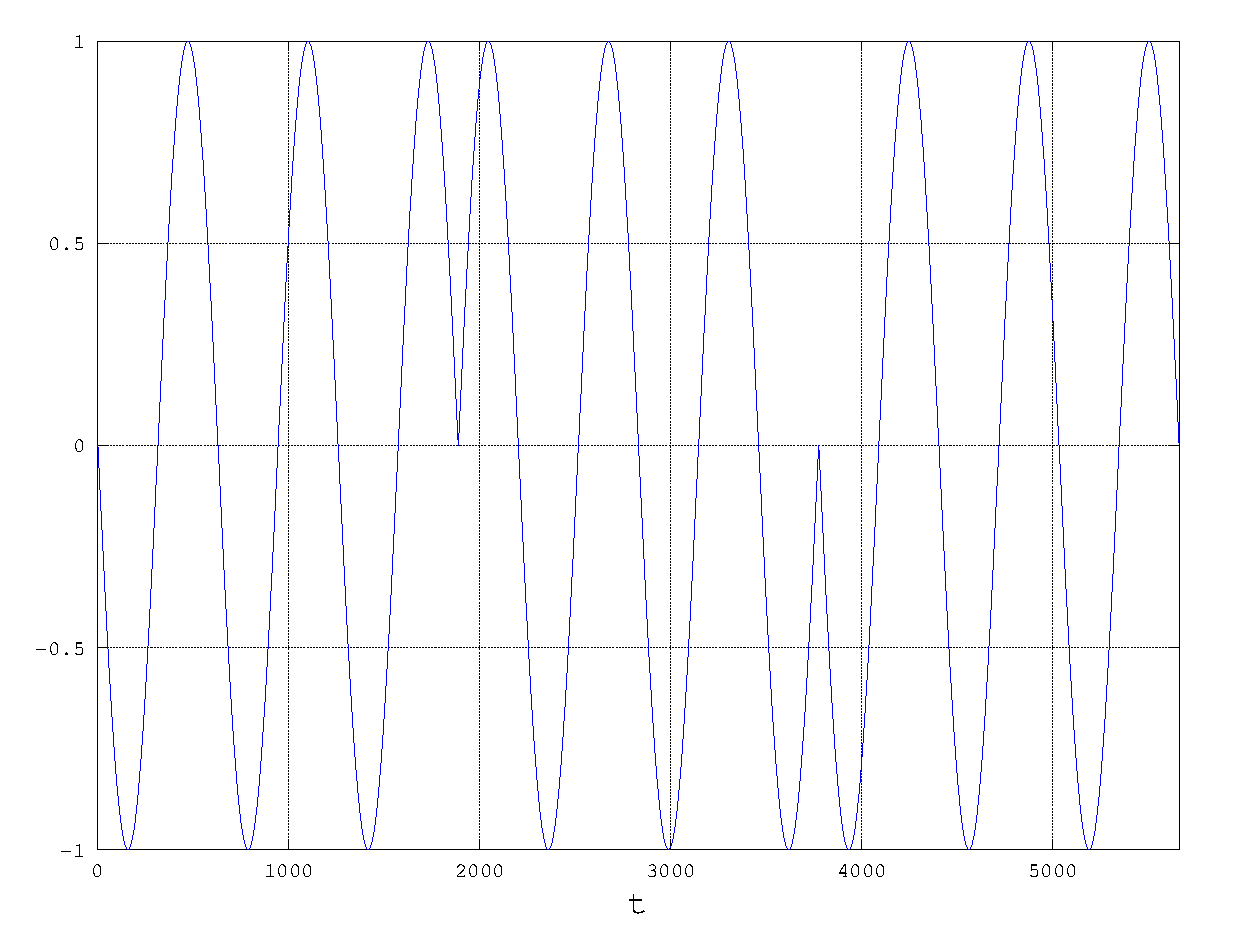
\includegraphics[width=1\linewidth]{bpsk.eps}}
\caption{Сигнал с модуляцией ДФМ}
\label{pic:sec1_bpsk}
\end{figure}
На рисунке \ref{pic:sec1_bpsk} представлена несущая, модулированная ДФМ.

Демодуляция производится повторной модуляцией принятого сигнала с синхронизированной копией ПСП ${C_k(t - \tau)}$, где
${\tau}$ - оценка фазы ПСП. При идеальной синхронизации входного сигнала, представленной выражением \ref{eq:gps_signal_phase},
c локальной копией ПСП, после демодуляции получаем (для простоты значение ${\tau}$ принято равным 0):
\begin{center}
\begin{eqnarray}
	\label{eq:gps_signal_modulated}
	s_k(t) & = & A C^2_k(t)\cos(\omega_{c}t) \nonumber \\
	& = & A \cos(\omega_{c}t)
\end{eqnarray}
\end{center}
Таким образом, на выходе демодулятора получается сигнал с суженным спектром. Следует отметить, что правильная оценка фазы ${\tau}$
является одной из основных задач при детектировании сигнала, так как ПСП имеет пик корреляции только в пределах центрального пика
АКФ \cite{gold-ieee}. При неверной оценке фазы ПСП в результате демодуляции спектр
ШПС не будет сужен, что может привести к ошибочным результатам на следующих этапах: вычислении ОСШ и принятии решения
о наличии или отсутствии искомого сигнала в смеси. 

\begin{figure}[H]
\center\scalebox{0.5}{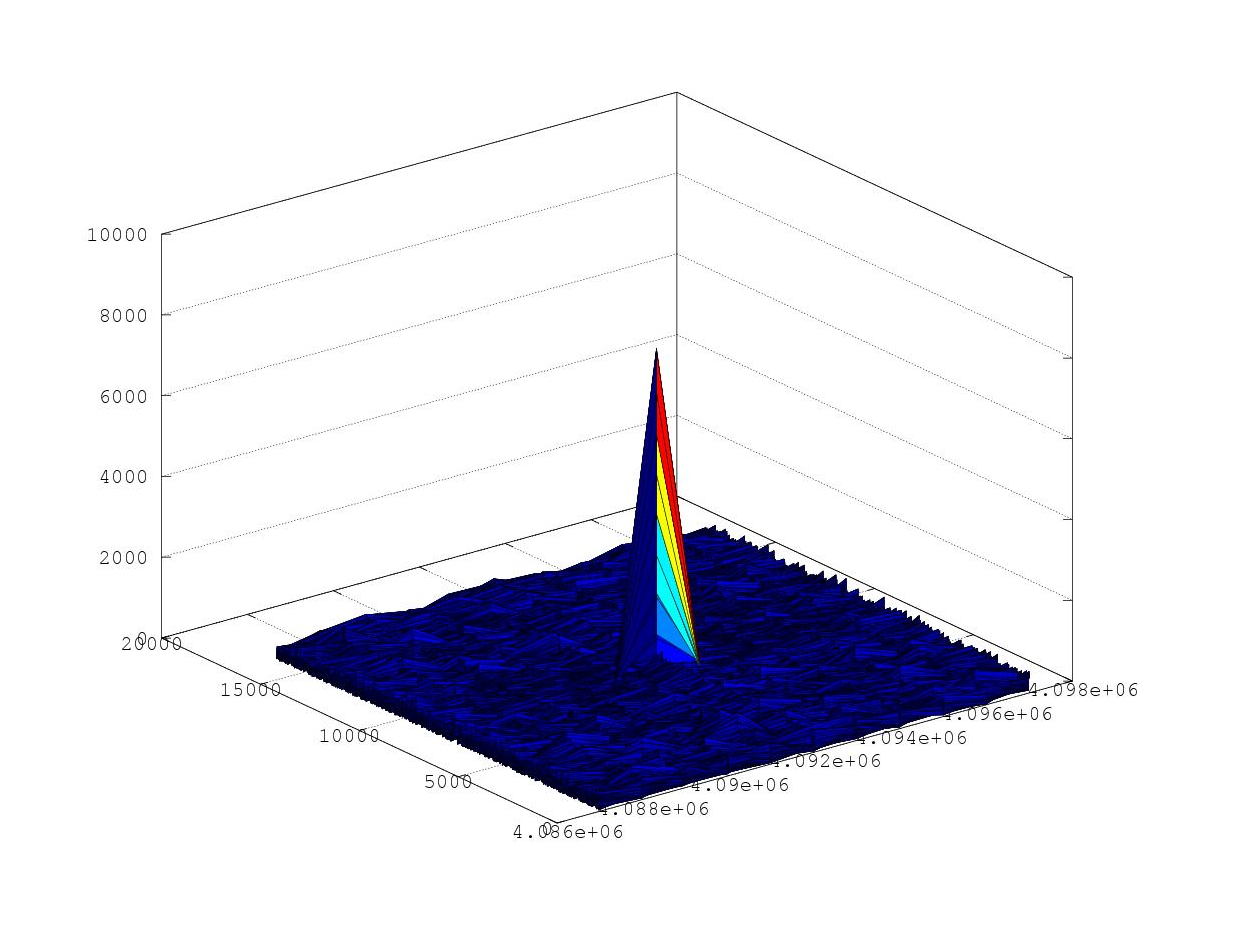
\includegraphics[width=1\linewidth]{corr_peak.eps}}
\caption{График ФН}
\label{pic:corr_peak}
\end{figure}

Задача поиска сигнала сводится к устранению неопределенности по двум параметрам: центральной частоте его спектра
и фазе ПСП. На рисунке \ref{pic:ambiguity_region} представлена область неопределенности. Можно заметить, что сечение
области неопределенности плоскостью ${f}$ представляет собой КФ сигнала. Поиск сигнала соответствует поиску и
оценке основного пика КФ.

\begin{figure}[H]
\center\scalebox{0.5}{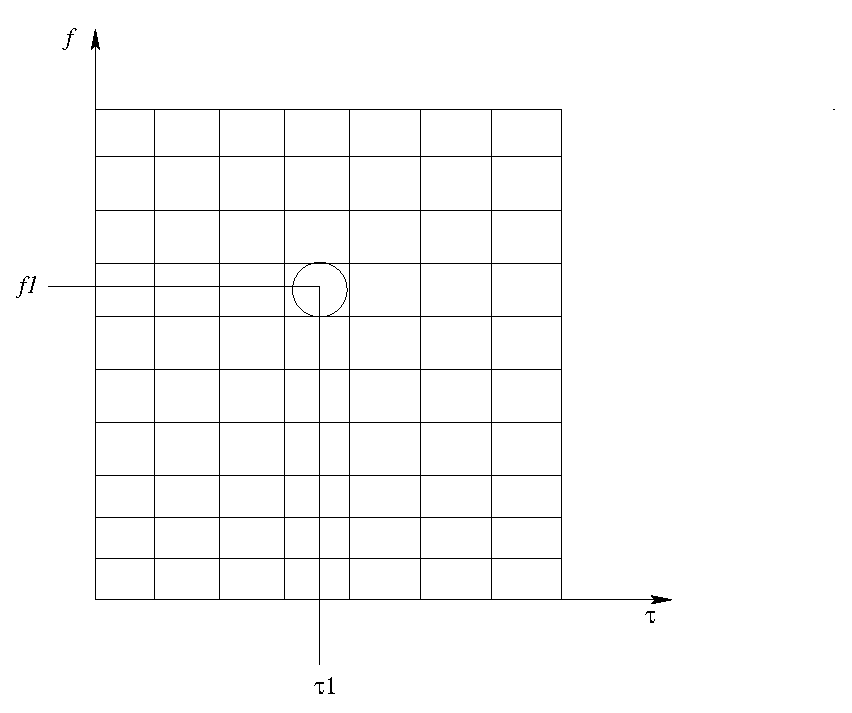
\includegraphics[width=1\linewidth]{ambiguity_region.eps}}
\caption{Область неопределенности}
\label{pic:ambiguity_region}
\end{figure}

\subsubsection{Модели помех}
\label{l:noise_model}
Обнаружение и распознавание помех всегда происходит в условиях действия помех и, решая задачу оптимизации приема,
необходимо иметь в виду определенные модели помех. Основной помехой является флуктуационная с нормальным
распределением мгновенных значений и широким равномерным энергетическим спектром. Такие помехи характеризуются
плотностью мощности ${N_n}$ на входе схемы оптимальной обработки \cite{pestryakov-book}.

Вторым видом помех, оказывающих
большое влияние на прием сигналов, являются помехи, связанные с рассеянным или многолучевым распространением
радиосигналов. Многолучевое распространение радиоволн, можно рассматривать или как фактор, обуславливающий
наличие дополнительных помех в виде сигналов, аналогичных тому, который рассматривается как основной, но с другой
задержкой, или как фактор изменяющий статистические характеристики параметров принимаемого сигнала,
обуславливая случайность амплитуды \cite{pestryakov-book}.

Третьим видом помех, характерных для систем связи, использующих ШПС, являются помехи от шумоподобных сигналов,
принадлежащих другим адресам (каналам). Эти помехи определяются тем, что при использовании ШПС для разделения
сигналов по форме (кодовое разделение) сигналы, принадлежащие другим адресам, не являясь идеально ортогональными,
создают помехи. Сумма нескольких шумоподобных сигналов дает результирующий процесс, близкий к нормальному шуму,
поэтому помеху, создаваемую многими ШПС, во многих случаях можно рассматривать как нормальный шум с ограниченным
равномерным спектром и ограниченной мощностью \cite{pestryakov-book}.

Мощность помех подвергается значительным изменениям; это относится и к флуктуационным естественным помехам, так как
изменяются собственные шумы приемника, помехи, создаваемые атмосферой и космосом, усиление приемного устройства
и т.п. Следовательно, для основного вида помехи ее плотность мощности ${N_n}$ является случайной величиной.

В системе Navstar GPS можно выделить 6 источников помех \cite{parkinson_1996}:
\begin{itemize}
	\item {данные эфемерид - ошибки в позициях спутников;}
	\item {часы спутника - ошибки в переданных данных о времени;}
	\item {ионосфера - ошибки в коррекции псевдодальностей обусловленных ионосферными эффектами;}
	\item {тропосфера - ошибки в коррекции псевдодальностей обусловленных обусловленных тропосферными эффектами;}
	\item {многолучевость - эффект отраженных сигналов принятых антенной;}
	\item {приемник - ошибки в измерениях обусловленные термальным шумом, точностью ПО и т.д.}
\end{itemize}

Так как данные виды помех влияют только на точность определения координат, мы можем рассматривать упрощенную модель
канала, где все данные виды помех не рассматриваются отдельно. Более углубленные модели канала можно найти в
источниках: упрощенная модель канала с сигналом на промежуточной частоте \cite{lei_dong_phd}, модель многолучевого
распространения \cite{hannah_phd}, а так же \cite{burns_model, corbell_model, crs_model, brown_model}.
 
\subsection{Классическая постановка задачи}
\label{sec1_FIXME}

Из литературы по теории автоматических систем, например \cite{pugachev} (глава 10.1), известна классическая постановка
задачи задачи теории оптимальных систем. "На практике часто приходится решать задачу проектирования системы, когда
требуется определить характеристики системы таким образом, чтобы она имела наибольшую точность при данных условиях.
Систему обеспечивающую наибольшую возможную точность с какой-нибудь определенной точки зрения среди всех систем
заданного класса, обычно называют оптимальной" \cite{pugachev}.

В одной из постановок данной задачи \cite{pugachev} (глава 10.1), система считается полностью неизвестной
и требуется определить ее оператор так, чтобы она была оптимальной с точки зрения принятого критерия качества. Эта
задача сводится к определению с наибольшей возможной точностью некоторых параметров, от которых зависит принимаемый
сигнал. Но при этом важно учитывать не только точность, но и другие факторы, так как проектируемая система должна
удовлетворять многим, часто противоречивым требованиям. В виду приведенных факторов, обычно представляет собой
ряд компромиссных решений, удовлетворяющих всем предъявляемым к системе требованиям.

\subsection{Статистические критерии оптимальности}
Точность автоматической системы обычно характеризуется математическим ожиданием и дисперсией ее ошибки.
Математическое ожидание представляет собой систематическую ошибку системы в данных условиях, а дисперсия
характеризует уровень случайных ошибок \cite{pugachev} (глава 10.2). Так как в различных условиях работы
системы, которые встречаются случайно систематическая ошибка тоже является случайной, за критерий качества
системы при ее проектировании обычно принимают второй начальный момент ошибки - математическое ожидание
квадрата ошибки ошибки:
\begin{center}
\begin{equation}
	\label{eq:stat_err_prob}
	\eta = M[e^2(t)]
\end{equation}
\end{center}
Положительный квадратный корень из этой величины называют средней квадратичной ошибкой системы. Таким образом,
оптимальной системой обычно считают такую систему, которая имеет минимальную среднюю квадратичную ошибку.

Критерий минимума средней квадратичной ошибки является простейшим с математической точки зрения и обычно приводит
к наиболее простым методам определения оптимальных систем. Однако далеко не во всех задачах он может служить мерой
качества системы. Поэтому нельзя ограничиваться методами нахождения оптимальных систем по критерию минимума средней
квадратичной ошибки.

В случаях, когда необходимо проектировать следящую систему, приходится учитывать возможность срыва слежения,
который заключается в том что система перестает работать, если ее ошибка превосходит по абсолютной величине некоторый
уровень. При проектировании таких систем целесообразно принять за критерий качества вероятность срыва слежения. При
этом оптимальной считается такая система, которая обеспечивает минимум вероятности срыва слежения. Если срыв слежения
происходит в случае, когда абсолютная величина ошибки превосходит уровень $a$, то критерий минимума вероятности ошибки
слежения можно представить \cite{pugachev} (глава 10.2):
\begin{center}
\begin{equation}
	\label{eq:prob_lost_signal}
	p = P(e(t) > a) = min
\end{equation}
\end{center}

%Так же применяют метод вычисления среднего риска $R$, как математического ожидания
%от функции потерь $l(Y, Y_T)$ (подробнее \cite{pugachev} глава 10.2):
%\begin{center}
%\begin{equation}
%	\label{eq:prob_lost_func}
%	R = M(l(Y, Y_T))
%\end{equation}
%\end{center}
%где ${Y(t)}$ - все возможные реализации выходного сигнала, ${Y_T(t)}$ - требуемый выходной сигнал.


\subsection{Введение обозначений}
В предыдущих разделах была рассмотрена подробно структура систем с ШПС, применяемого в системе Navstar GPS. В данном разделе
будут введены обозначения для дальнейшего использования в данной работе.

Обозначим модель входного СНС для ${K}$ - источников как:
\begin{center}
\begin{equation}
	\label{eq:gps_model_1}
	s(t) = \sum_{k=1}^{K}{A_{k}C_{k}(t-\tau_k)D_{k}(t-\tau_k))\cos(\omega_{c}t + \phi_k)}
\end{equation}
\end{center}
где: ${A}$ - амплитуда сигнала, ${C_k(t)}$ - ПСП для ${k}$ - сигнала, ${D_k(t)}$ - данные, а ${\omega_{k}}$ - частота несущей сигнала.

\subsection{Оптимальный приемник сигнала}
Оптимальный приемник сигнала состоит из оптимальной обработки сигнала и операции сравнения (или принятия решения). Стоит отметить,
что схема оптимальной обработки сигнала не зависит от операции принятия решения, так как как операция принятия решения зависит от
априорных сведений (например $A$, $\phi_k$ в \ref{eq:gps_model_1}). Для реализации оптимального приемника при неизвестных априорных
сведениях схема оптимальной обработки сигнала останется старой, а вот правила выбора порога будут другими \cite{pestryakov-book}.

При обнаружении сигнала некоторое время производится наблюдение за входной смесью, в результате чего формируется реализация $s(t)$ (индекс $k$
опущен, так как для простоты изложения рассматривается один сигнал после операции умножения сигнала на ПСП источника $k$) или
выборка $s_{1}s_{2}...$ Данная реализация может содержать только помеху или смесь сигнала и помехи. Для получения аналитического
выражения для оптимального алгоритма обработки смеси при принятии решения о пришествии или отсутствии сигнала,
нужно вероятностно описать протекание за длительное время смеси при наличии в ней сигнала и помехи или действия только помехи. Для
этого нужно выписать функции распределения смеси, содержащей только флуктуационную помеху в виде нормального гауссового шума \cite{pestryakov-book}:
\begin{center}
\begin{eqnarray}
	\label{eq:just_noise}
	w(x_{1}x_{2}.../n) & = & \frac{1}{(2\pi\sigma_{n}^{2})^{k_n/2}}\exp[-\frac{1}{2\sigma_{n}^{2}}\sum_{j=1}^{k_n}x_{j}^2] = \\
			& = & \frac{1}{(2\pi\sigma_{n}^{2})^{k_n/2}}\exp[-\frac{1}{N_n}\int_{0}^{T_n}x^2(t)] \nonumber
\end{eqnarray}
\end{center}
где $k_n=T_n/\tau_{kn}=2T_nf_{n}$ - объем выборки; ${T_n}$ - время наблюдения; ${f_{n}}$ - высшая частота в спектре помехи;
${N_n}$ - плотность мощности помехи; ${\sigma_{n}^{2}}$ - дисперсия помехи; ${t_{kn}}$ - интервал корреляции помехи.

Смесь сигнала и помехи может быть записана как:
\begin{center}
\begin{equation}
	\label{eq:signal_and_noise}
	x(t) = s(t, \beta_1, \beta_2, ...) + n(t)
\end{equation}
\end{center}
Смесь является случайным процессом. Условная многомерная функция распределения значений смеси при условии, что параметры
сигнала ${\beta_1, \beta_2, ...}$ имеют определенное значение, равна:
\begin{center}
\begin{eqnarray}
	\label{eq:signal_and_noise2}
	w(x_{1}x_{2}...x_{k}/\beta_1 \beta_2 ..., n) & = & \\
	& = & \frac{1}{(2\pi\sigma_{n}^{2})^{k_n/2}}\exp[-\frac{1}{N_n}\int_{0}^{T_n}[x(t) - s(t, \beta_1, \beta_2, ...)]^2 dt] \nonumber
\end{eqnarray}
\end{center}

Так как шумовая компонента является случайным процессом, ее статистические характеристики могут быть описаны как:
\begin{center}
\begin{equation}
	%\label{eq:signal_and_noise}
	w(\beta_1, \beta_2, ...)
\end{equation}
\end{center}

Многомерная функция распределения вероятностей для смеси сигнала и шума примет вид:
\begin{center}
\begin{equation}
	\label{eq:w_sn}
	w(x_{1}x_{2}.../sn) = \int \int ... \int w(\beta_1, \beta_2, ...)w(x_{1}x_{2}.../ \beta_1, \beta_2, ..., sn) d\beta_1 d\beta_2 ...
\end{equation}
\end{center}

В случае сигнала с заранее известными параметрами выражение \ref{eq:w_sn} примет вид:
\begin{center}
\begin{eqnarray}
	\label{eq:w_sn2}
	w(x_{1}x_{2}...x_{k}/sn) & = & \\
	& = & \frac{1}{(2\pi\sigma_{n}^{2})^{k_n/2}}\exp[-\frac{1}{N_n}\int_{0}^{T_n}[x(t) - s(t)]^2 dt] \nonumber
\end{eqnarray}
\end{center}

После преобразований получаем, что принятие гипотезы о наличии сигнала в смеси сопровождается минимальным рисском, при условии выполнения:
\begin{center}
\begin{eqnarray}
	\label{eq:func_likehood}
	l(x) = \frac{w(x_{1}x_{2}...x_{k}/sn)}{w(x_{1}x_{2}...x_{k}/n)} > Threshold 
\end{eqnarray}
\end{center}
где ${Threshold}$ - порог, а ${l(x)}$ - отношение правдоподобия.

Приведенное доказательство заимствовано из \cite{pugachev} (глава 13.4)

\newpage
